\chapter{Liquid Argon Detectors at the Intensity Frontier}\label{ch:2}
{\raggedleft ``\emph{Don't you know, honey,} \par}
{\raggedleft \emph{Ain't nobody ever gonna love you, the way I try to do?}"\par}
{\raggedleft -- Janis Joplin,  1971 -- \par}%Cry Baby,
\vspace{0.5cm}

In the next few years, LArTPCs will  be the tools to answer some of the burning questions in neutrino physics today.  This chapter illustrates the operational principles of this detector technology, as well as the scope of the key detectors in the US liquid argon program -- SBN, DUNE and LArIAT.


\section{The Liquid Argon Time Projection Chamber Technology}
In this section, we outline an extremely brief history of Time Projection Chambers as particle detectors, focusing on their incarnation as argon detectors for neutrino physics. We further describe the working principles of Liquid Argon Time Projection Chambers, leading  to the description of the event reconstruction in LArTPC.

\subsection{TPCs, Neutrinos \& Argon}
David Nygren designed the first Time Projection Chamber (TPC) in the late 1970s~\cite{FirstTPC} for the  PEP-4 experiment, a detector  apt to study electron-positron collisions at the PEP storage ring at the SLAC National Accelerator Laboratory.
From the original design  in the seventies -- a cylindrical chamber filled with methane gas -- the TPC detector concept has seen many incarnations, the employment of several different active media and a variety of different particle physics applications, including, but not limited to the study of electron/positron storage rings (e.g. PEP4, TOPAZ, ALEPH and DELPHI), heavy ions collisions in fixed target and collider experiments (e.g. EOS/HISS and ALICE ), dark matter (ArDM), rare decays and capture (e.g. TRIUMP, MuCap),  neutrino detectors and nucleon decay (ICARUS, SBN, DUNE), and neutrino less double beta decay (Next, EXO-200\/nEXO). A nice review of the history of TPCs and working principles is provided in \cite{0034-4885-73-11-116201}.

Several features of the TPC technology make these detectors a more versatile tool compared to other ionization detectors and explain such a wide popularity. TPCs are the only electronically read detector which deliver simultaneous  three-dimensional track information and a measurement of the particle energy loss. Leveraging on both tracking and calorimetry,  particle identification (PID) capabilities are enhanced  over a wide momentum range. 

Historically, the active medium in ionization detectors has been in the gaseous form. Willis and Radeka first proposed the use of liquid-argon ionization chambers as total-absorption detectors in their pioneer work of 1974 \cite{WILLIS1974221}
Carlo Rubbia imported this concept to neutrino detection with the ICARUS experiment \cite{Rubbia:1977zz}, in 1977.  Using nobles elements in the liquid form for neutrino detectors is advantageous for several reasons.  The density of liquids is $\sim$1000 times greater than gases, augmenting the number of targets for neutrino's interaction in the same volume, in a effort to balance the smallness of neutrino cross section. Since the energy loss of charged particle is proportional to the target material density, as shown in the Bethe-Block equation (eq. \ref{eq:BB}), the increased density reflects into a proportionally higher energy loss, enhancing the calorimetry capability of detectors with a liquid active medium. Additionally, the ionization energy of liquids is smaller than gasses by the order of tens of eV. Thus, at the passage of charged particles, liquids generally produce more ionization electrons than gases for the same deposited energy, forcing the particles to deposit more energy in a shorter range. The downside of using noble liquid elements in experiments is that they require expensive cryogenic systems to cool the gas until it transitions to its liquid form.
The properties of liquid argon in comparison liquid xenon -- a popular choice for dark matter and neutrinoless double beta decay detectors -- are summarized in table \ref{tab:properties}.  Albeit xenon would be more desirable than argon given some superior properties such as lower ionization energy and higher density and light yield, argon relative abundance abates the cost of argon compared to xenon, making argon a more viable choice for the construction of ton  (and kilo-ton) scale neutrino detectors. 




\begin{table}[]
\centering
\begin{tabular}{|l|c|c|}\hline
Element & LAr & LXe \\
\hline
\hline
Atomic Number &  18 &54 \\
Atomic weight A & 40  & 131\\
Boiling Point Tb at 1 atm & 87.3 K & 165.0 K\\
Density  & 1.4 g/cm$^3$& 3.0 g/cm$^3$\\
Radiation length  & 14.0 cm& 2.8 cm \\
Moliere Radius  &10.0 cm& 5.7 cm\\
Work function  & 23.6 eV&15.6 eV\\
Electron Mobility at $E_{field} =10^4$ V/m &0.047 m$^2$/Vs& 0.22 m$^2$/Vs\\
Average dE/dx MIP  & 2.1 MeV/cm&3.8 MeV/cm\\
Average Scintillation Light Yield & 40000 $\gamma$/MeV&42000 $\gamma$/MeV\\
Scintillation $\lambda$  &128 nm&175 nm\\
\hline
\end{tabular}
\caption{LAr, LXe summary of properties relevant for neutrino detectors.}
\label{tab:properties}
\end{table}


LArTPCs are some times referred as to ``electronic" bubble-chambers, for the similarity in the tracking and energy resolution which is coupled with an electronic readout of the imaging information in LArTPCs. Compared to these historic detectors however, LArTPC bestow tridimensional tracking, calorimetry and a self triggering mechanism provided by the scintillation light in the liquid argon.  An event display of a $\nu_\mu$ CC interaction candidate in the MicroBooNE detector is shown in picture \ref{fig:NuEvd} to display the level of spatial details these detectors are capable of; the color scale of the image is proportional to the energy deposited, hinting to these calorimetry capabilities of the detectors.
\begin{figure}[hbpt]
\centering
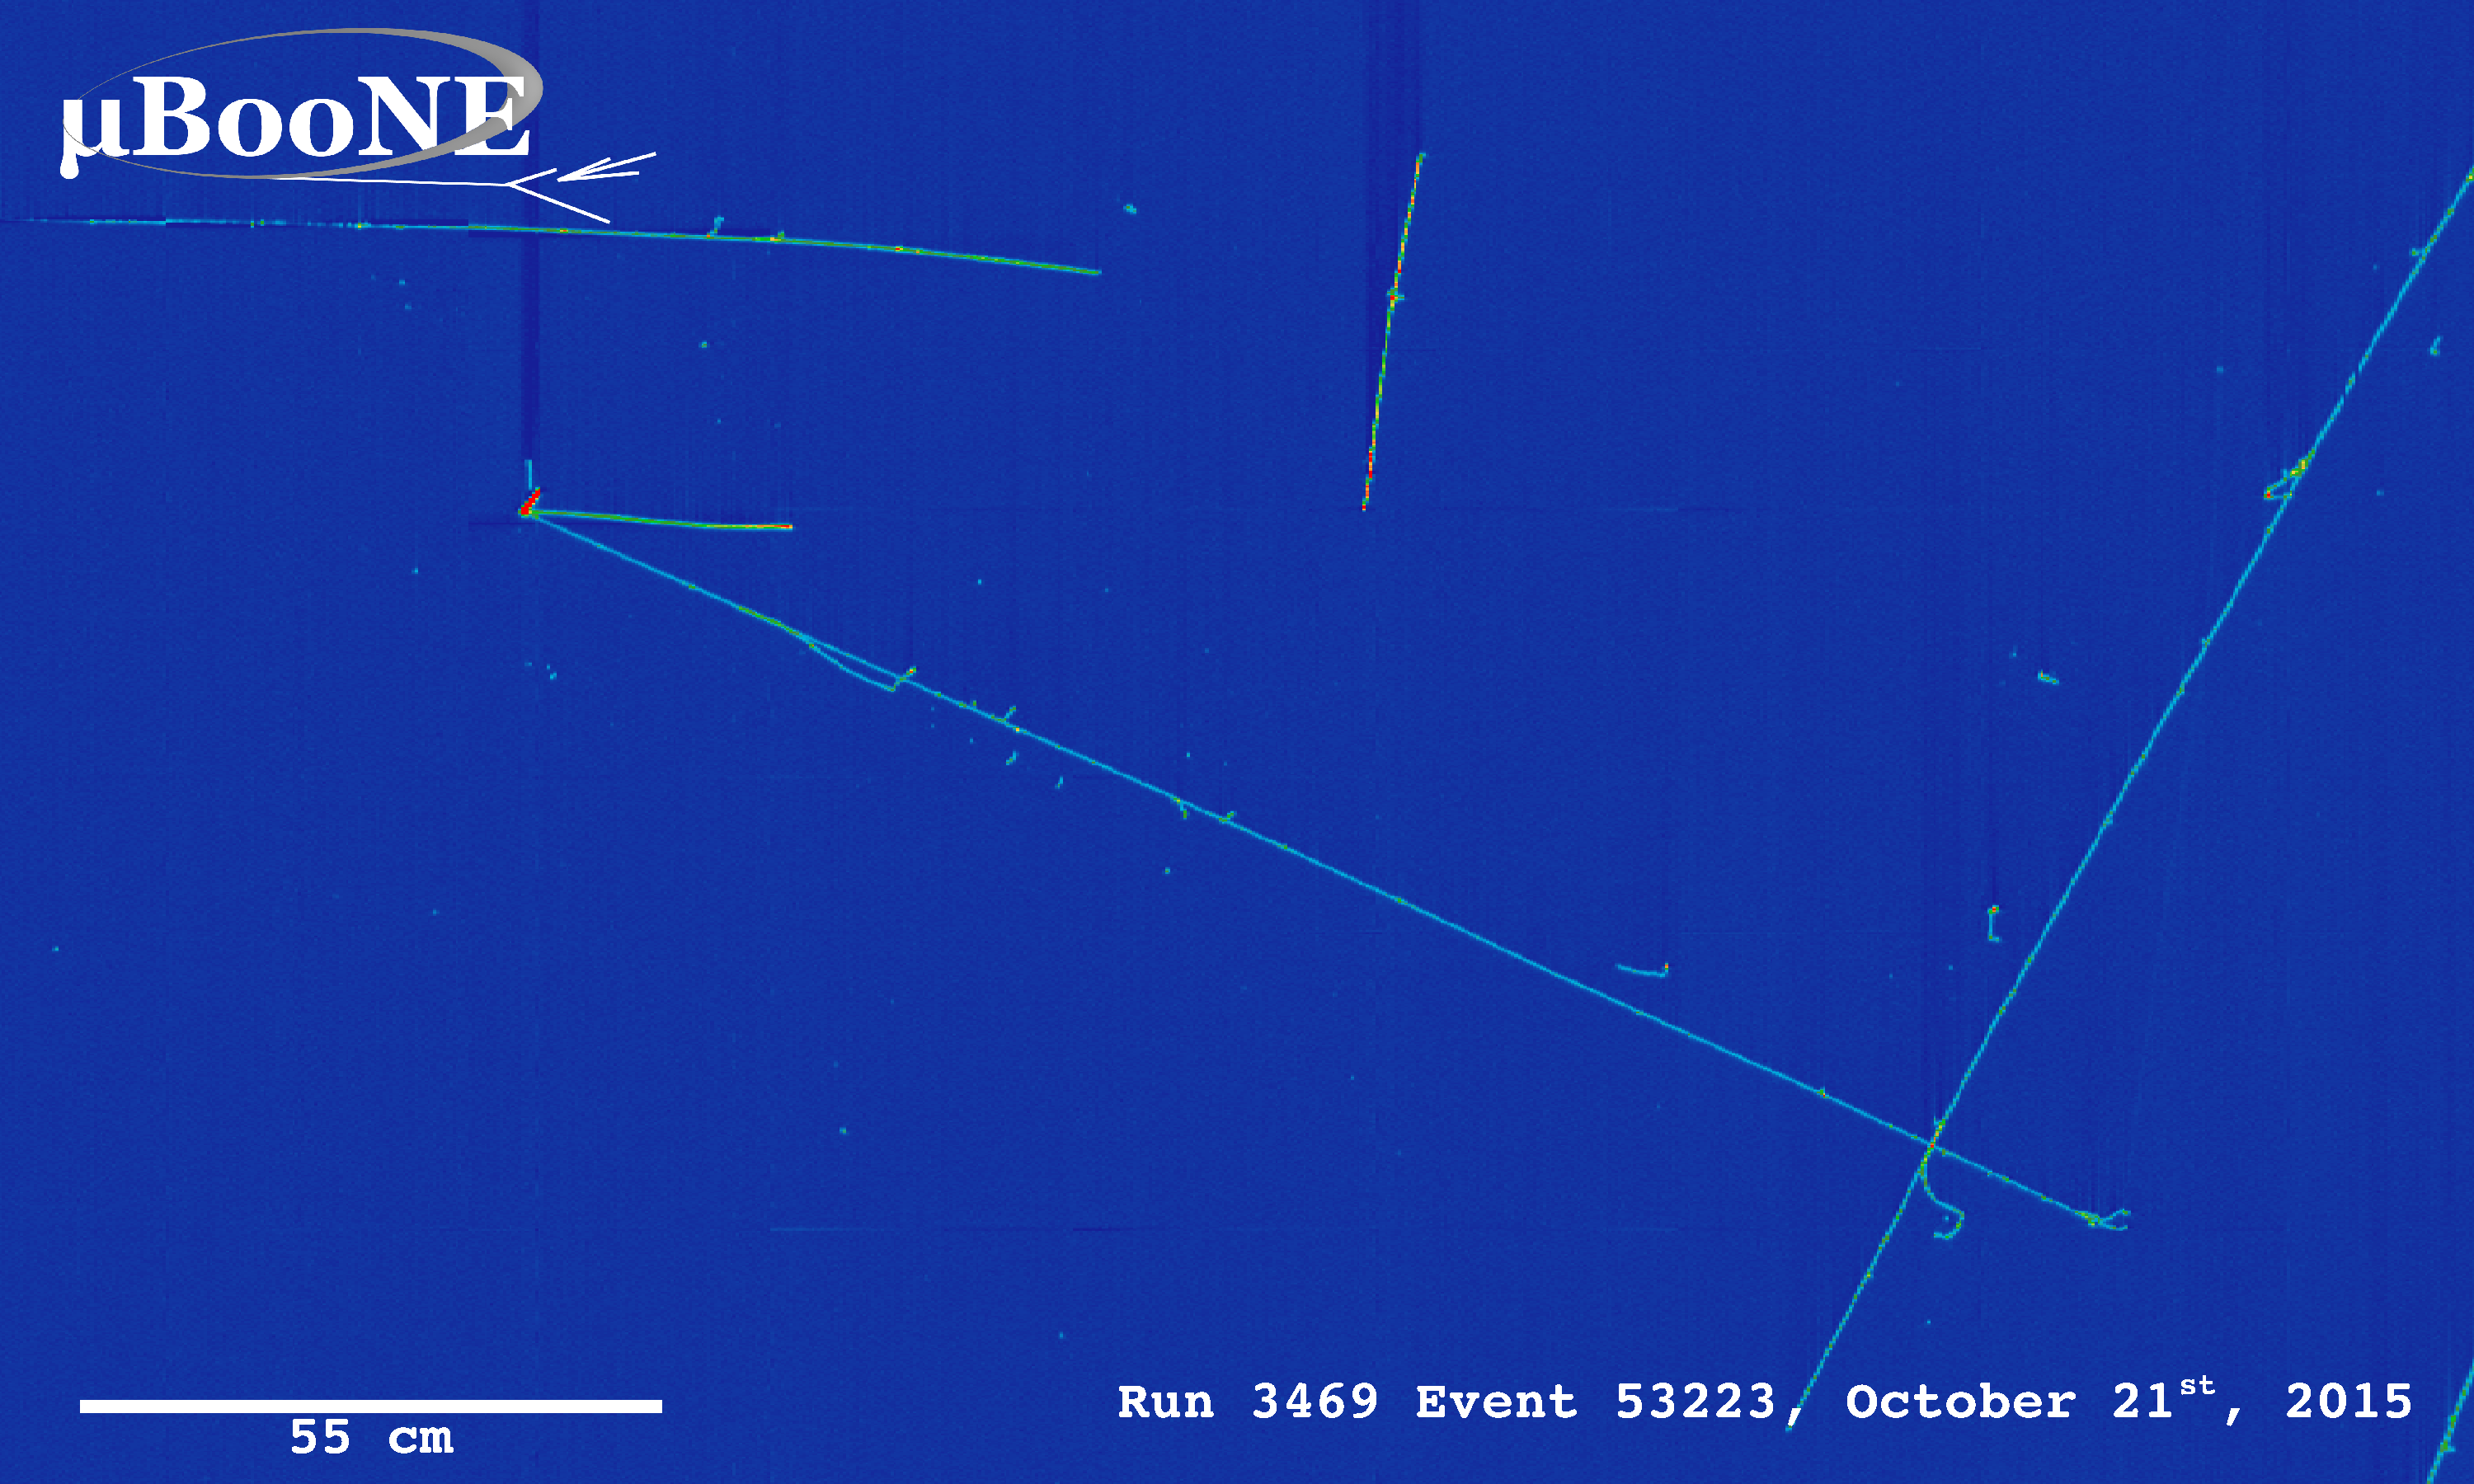
\includegraphics[width=\textwidth]{Chapter-2/Images/run3469_subrun1064_event53223_col.pdf}
\caption{Event display of a $\nu_\mu$ CC interaction candidate in the MicroBooNE detector.}
\label{fig:NuEvd}
\end{figure}



\subsection{LArTPC: Principles of Operation}\label{sec:LArTPCWorkingPrinciple}

\begin{figure}[hbpt]
\centering
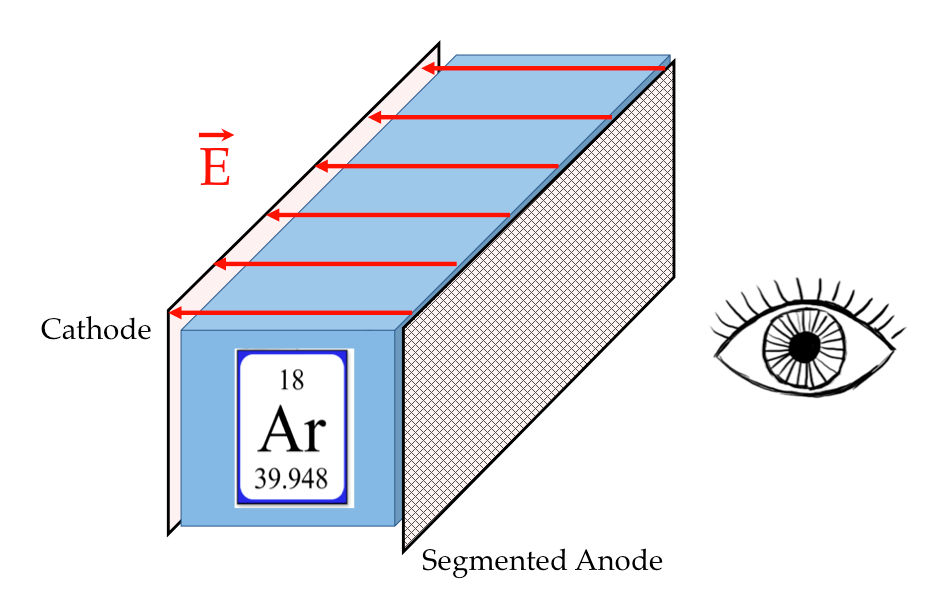
\includegraphics[width=\textwidth]{Chapter-2/Images/Cartoon.png}
\caption{A cartoonish sketch of a LArTPC.}
\label{fig:cartoon}
\end{figure}


To the bare bones, a LArTPC is a bulk of liquid argon sandwiched in a flat capacitor, equipped with a light collection system, as the cartoon in \ref{fig:cartoon} shows. A uniform electric field of the order of 500 V/cm is maintained constant between the conductive faces and field shaping rings are used to avoid fringing fields. The anode is sensitive to ionization charge and it is usually made of two or more planes segmented into several hundreds parallel sense wires a few millimeters apart; different geometries for the anode segmentation are under study \cite{1748-0221-8-07-P07002}. 

Argon ionization and scintillation are the processes leveraged to detect particles in the LArTPC active volume.  When a ionizing radiation traverses the argon active volume it leaves a trail of ionization electrons along its trajectory and it excites the argon producing scintillation light -- details on the production and detection of ionization charge and scintillation light are provided in \ref{sec:light}. The optical detector sees the argon scintillation light in matters of nanoseconds. This flash of light determines the start time of an event in the chamber, $t_0$. The uniform electric field drifts the ionization  electrons from the production point towards the anode in order of hundreds of microseconds or more depending on the chamber dimensions\footnote{The ionized argon also drifts, but  in the opposite directions compared to the electrons. Since the drift time is proportional to the particle mass,  the ions' drift time is much longer than the electrons'.  Ionized argon is collected on the cathode which is not instrumented, so it is not used to infer information about the interactions in the chamber.}. The anode sense wires see either an induced current by the drifting ionization charge (on induction planes) or an injection of such charge (collection plane).    An appropriate choice of the voltage bias on each wire plane assures ideal charge transparency, so that all the ionization charge is collected on the collection plane and none on the induction planes.  

The arrival time of the charge on the anode sense wires is used to measure the position of the original ionizing radiation in the drift direction. In fact, since the constant electric field implies that the drift velocity is also constant, the position of the original ionization is simply given by the multiplication of the drift velocity by the drift time, where the ``drift time" is the difference between $t_0$ and the charge arrival time on the wire planes. The spatial resolution on this dimension is limited by the time resolution of the electronics or by longitudinal diffusion of the electrons.
The spatial information on the different wire planes maps a bi-dimensional projection of the interaction pattern in the plane perpendicular to the drift direction. The spacial resolution on this dimension is limited by the transverse electron diffusion in argon and by the grain of the anode segmentation, i.e. the spacing between the wires in the sense planes \cite{DERENZO1974319}.  The off-line combination of the 2-D information on the wire planes with the timing information allows for the 3D reconstruction of the event in the chamber.

Since the charge deposited by the ionizing radiation is proportional to the deposited energy and the charge collected on the sense plane is a function of the deposited charge, LArTPCs allow the measurement of the energy deposit in the active volume. Effects due to the presence of free charge and impurities in the active volume, such as a finite electron lifetime, recombination and space charge, complicate the relationship between deposited and collected charge affecting the measurement of the particle's energy, as described in the next section.
 
\subsection{Liquid Argon: Ionization Charge}\label{sec:charge}
The mean rate of energy loss by moderately relativistic elementary charge particles heavier than electrons is well described by the modified Bethe-Bloch \cite{Patrignani:2016xqp} equation
\begin{eqnarray}
			- \frac{dE}{dx} = K z^2 \frac{Z}{A} \varrho \frac{1}{\beta^2} \left[ \frac{1}{2} \ln{\frac{2 m_e c^2 \beta^2 \gamma^2 T_{max}}{I^2}} - \beta^2 - \frac{\delta}{2}\right] ,
			\label{eq:BB}
\end{eqnarray}
where  $z$ is the number of unit charge of the ionizing radiation, $Z$, $A$  and $\varrho$ are the atomic number, mass number and density of the medium,  $m_e$  is the electron mass, $\gamma = \frac{\beta}{\sqrt{1-\beta^2}} $ is the Lorentz factor of the ionizing radiation,  $T_{max}$ is the maximum kinetic energy which can be
imparted to a free electron in a single collision, $I$ is the mean excitation energy on eV,  $\delta$ is the  density correction and $K = 0.307 075 \text{ MeV g}^{-1}\text{ cm}^2$ is a numerical conversion factor. The Bethe-Bloch treats the energy loss by an ionizing radiation via quantum-mechanical collisions producing ionization or an excitation in the medium as an uniform and continuous process. The density correction  terms becomes relevant for incident particle with high energy, where screening effects due to the polarization of the medium by high energy particles occur.

Excitation and ionization of the detector medium occur in similar amounts. Since the ionizing collisions occur randomly, we can parametrize their number $k$ in a segment of length $s$ along the track  with a Poissonian function
\begin{equation}
P(k) = \frac{s^k}{k! \lambda^k} e^{-s/ \lambda }, 
\end{equation}
where $\lambda = 1/N_{e}\sigma_i$, with $N_{e}$ being the electron density of $\sigma_i$ the ionization cross-section per electron.  About 66\% of the ionizing collisions in argon produce only a single electron/ion pair \cite{0034-4885-73-11-116201}; in the other cases, the transferred kinetic energy is enough for the primary electron to liberate one or more secondary electrons, which usually stay close to the original pair.  
Occasionally, electrons can receive enough energy to be ejected with high energy, forming a so-called ``$\delta$-ray": a detectable  short track off the particle trajectory, as shown in figure \ref{fig:delta}. 
The average number of $\delta$-ray  with energy E$>$E$_0$ per cm follows the empirical form
\begin{equation}
P(E>E_0) \sim \frac{y}{\beta^2 E_0},
\end{equation}
where $y$ is an empirical factor depending on the medium (0.114 for  gaseous Ar), and $\beta$ is $v/c$.

\begin{figure}[hbpt]
\centering
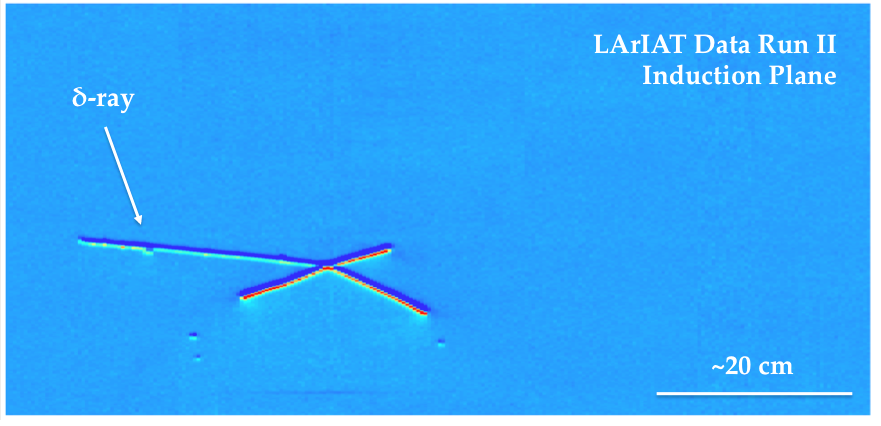
\includegraphics[width=\textwidth]{Chapter-2/Images/Delta.png}
\caption{Event display for a LArIAT pion absorption candidate on the induction plane, with highlighted delta ray.}
\label{fig:delta}
\end{figure}


		
\subsubsection{Purity \& Electron Life Time }
The presence of electronegative contaminants in liquid argon, such as oxygen $O_2$ and water $H_2O$, is particularly
pernicious, since these molecules quench the charge produced by the ionizing radiation.  Thus, amount of charge per unit of length $dQ/dx$ collected on the collection plane depends on the charge's production point in the detector: ionization produced  close to the cathode will see more impurities along its journey to the collection plane than ionization produced close to the anode, resulting in greater attenuation of its charge. As a result,  the amount of charge collected on the sense wires as a function of the traveled distance follows an exponential decay trend. The traveled distance is generally measured in terms of drift time and the  characteristic time constant of the exponential decay is called electron lifetime $\tau_e$. Figure \ref{fig:Elifetime} shows the typical life time for LArIAT data. The procedure to measure the electron lifetime in LArIAT is outlined in \cite{LArIATLifeTime}. LArIAT small drift distance (47 cm) allows for a relatively short electron life time. The life time for bigger detectors such as MicroBooNE, whose drift distance is 2.6 m, needs to be of the order of tens of milliseconds to allow a charge collection usable for physics analyses. Energy reconstruction in LArTPC applies a correction for the finite lifetime to calibrate the detector calorimetric response; details for LArIAT are provided in Section \ref{ch:energyCalibration}.

\begin{figure}[hbpt]
\centering
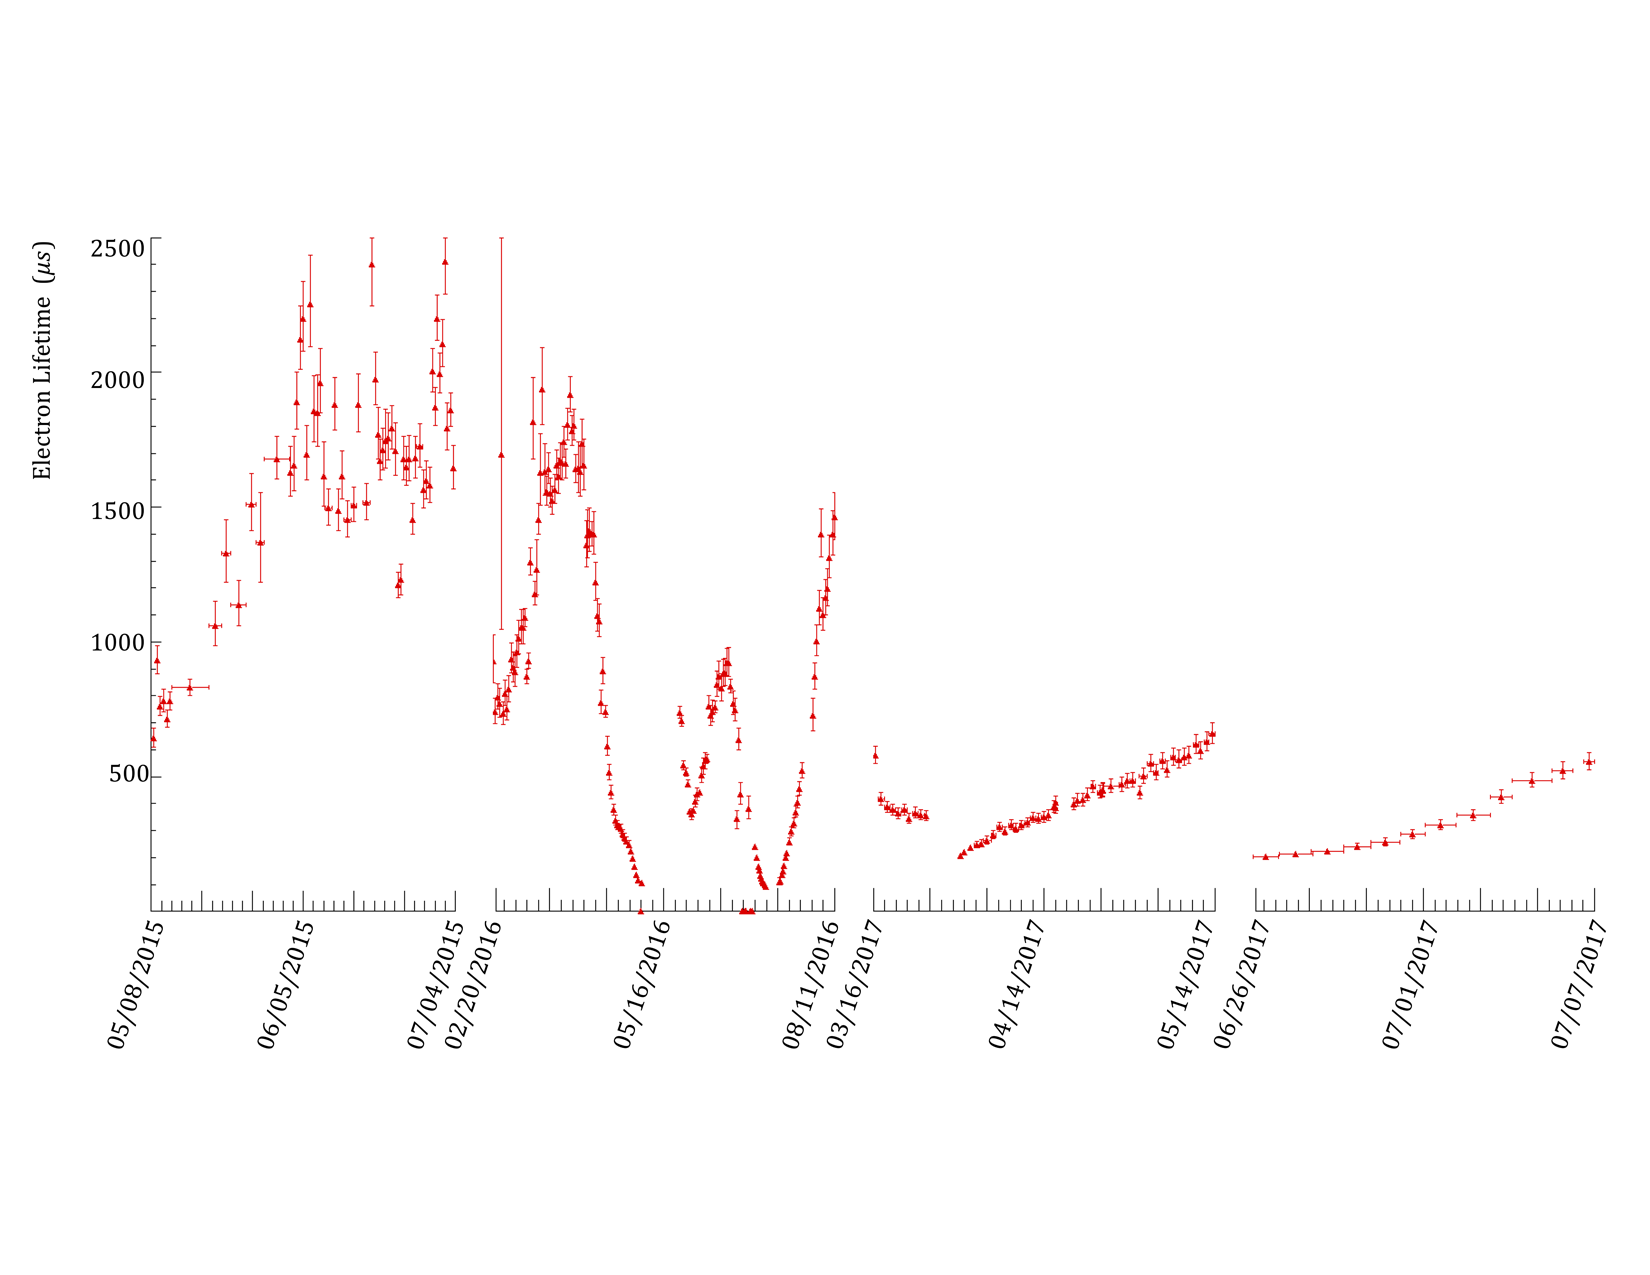
\includegraphics[width=\textwidth]{Chapter-2/Images/ELifetime.png}
\put(-98,260){\bf\tiny{LArIAT Preliminary}}
\caption{Electron lifetime during the LArIAT run period \cite{detectorPaper}.}
\label{fig:Elifetime}
\end{figure}


LArTPCs use  hermetically sealed and leak-checked vessels to abate the leakage and diffusion of contaminants into the system. The liquid argon filling of the volume occurs after the vessel is evacuated or purged with gaseous argon \cite{1748-0221-9-07-P07005} to reduce remaining gases in the volume. Even so, the construction of a pure tank of argon is unviable, as several sources of impurity remain.  In particular, impurities can come from the raw argon supply, the argon filtration system and from the outgassing from internal surfaces. Outgassing is a continuous diffusive process  producing contaminants, especially water, even after the vessel is sealed, particularly from materials in the ullage region\footnote{While the liquid argon low temperature reduces outgassing in the liquid, this process remains significant for absorptive material (such as plastic) above the surface of the liquid phase.}.  Since research-grade argon comes from the industrial distillation of air, the impurities with the highest concentration are nitrogen, oxygen and water, generally maintained under the 1 part per million level by the vendor.  Even so, a higher level of purity is necessary to achieve a free electron life time usable in meter scale detectors. Thus, argon  is constantly  filtered in the cryogenic system, which reduce the oxygen and water contamination to less than 100 parts per trillion. The filtration system depends on the size and drift distance of the experiment and, for experiments on several meters scale, it includes an argon recirculation system \cite{MicroBooNE-det}.

%% Life time value for LArIAT


\subsubsection{Recombination Effect}
After production, ionization electrons thermalize with the surrounding medium and may recombine with nearby ions. Recombination might occur either between the electron and the parent ion through Coulomb attraction, as described in the geminate theory  \cite{PhysRev.54.554}, or thanks to the collective charge density of electrons and ions from multiple ionizations in a cylindrical volume surrounding the particle trajectory, as described in the  columnar model \cite{Jaff1913}. 
Consideration on the  average electron-ion distance and the average ion-ion distance for argon show that the probability of geminate recombination is low; thus recombination in argon is mainly due to collective effects\cite{1748-0221-8-08-P08005}.  Since protons, kaons and stopping particles present a higher ionization compared to MIPs, recombination effects are more prominent when considering the reconstruction of energy deposited by these particles.

Theoretical descriptions of recombination based on the Birks model and the Box model are provided in \cite{0370-1298-64-10-303} and  \cite{PhysRevA.36.614}, respectively. The Birks model assumes a gaussian spatial distribution around the particle trajectory during the entire recombination phase and identical charge mobility for ions and electrons. The Box model also assumes that electron diffusion and ion mobility are negligible in liquid argon during recombination.
In these models, the fraction of ionization electrons surviving recombination is a function of the number of ion-electron pairs per unit length, the electric field, the average ion-electron separation distance after thermalization and the angle of the particle with respect to the direction of the electric field -- plus the diffusion coefficient in the Birks model. Given the stringent assumptions, it is perhaps  not surprising that these models are in accordance to data only in specific regimes: the Birks model is generally used to describe recombination for low dE/dx, the Box model for high dE/dX.
In LArTPC, the ICARUS and ArgoNeut experiments have measured recombination in \cite{Amoruso:2004dy} and \cite{1748-0221-8-08-P08005} respectively. Since LArIAT uses the refurbished ArgoNeut TPC and cryostat at the same electric field,  LArIAT currently corrects for recombination using the ArgoNeut measured recombination parameters in \cite{1748-0221-8-08-P08005}.


\subsubsection{Space Charge Effect}
Slow-moving positive argon ions created during ionization can build-up in LArTPC, causing the distortion of the
electric field within the detector. This effect, called  ``space charge effect" leads to a displacement in the reconstructed position of the signal ionization electrons. In surface LArTPCs the space charge effect is primarily due to the rate of ionization produced by cosmic rays which is slowly drifting in the chamber at all times. Surface LArTPC of the size of several meters are expected to be modestly impacted from the space charge effect, where charge build-up create anisotropy of the electric field magnitude of the order of  5\% at a drift field of 500 V/cm \cite{SpaceCharge}. The smallness of the LArIAT drift volume and its relatively high electric field are such that the effect of  space charge is expected to be negligible. 

%%%%%%%%%%%%%%%%%%%%%%%%%%%%%%%%%%%%%%%%%%%%%%%%%%%%%%%%%%%%%%%
%%%%%%%%%%%%%%%%%%%%%                     Light Detection             %%%%%%%%%%%%%%%%%%%%%%%%
%%%%%%%%%%%%%%%%%%%%%%%%%%%%%%%%%%%%%%%%%%%%%%%%%%%%%%%%%%%%%%%
\subsection{Liquid Argon: Scintillation Light }\label{sec:light}
Liquid argon emits scintillation light at the passage of charged particles. LArTPCs  leverage this property to determine when the ionization charge begins to drift towards the anode plane. %Scintillation light can also be used for particle identification, as discussed in the next sections.

\subsubsection{Scintillation Process}
Scintillation light in argon peaks in the ultraviolet at a 128 nm, shown in comparison to Xenon and Kypton in Figure  \ref{fig:ArLight}, from \cite{Morikawa1989}. The light yield collected by the optical detector depends on the argon purity, the electric field, the dE/dx and particle type, averaging at the tens of thousands of photons per MeV. 

\begin{figure}[hbpt]
\centering
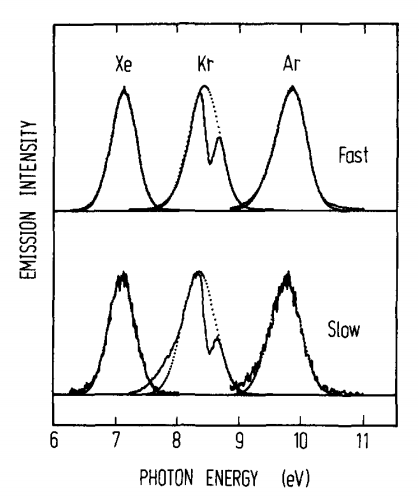
\includegraphics[scale=0.5]{Chapter-2/Images/Light.png}
\caption{Emission spectra of the fast and slow emission components in Xenon, Kypton and Argon according to \cite{Morikawa1989}. The dotted lines correspond to the Gaussian fits. }
\label{fig:ArLight}
\end{figure}




The de-excitation of Rydberg dimers in the argon is responsible for the scintillation light. 
Rydberg dimers exist in two states:  singlets and a triplets. The time constant for the singlet radiative decay is 6 ns, resulting in a prompt component for the scintillation light. The decay of the triplet is delayed by intersystem crossing, producing a slow component with a time constant of $\sim$~1500 ns.  ``Self-trapped exciton luminescence" and  ``recombination luminescence" are the two processes responsible for the creation of the Rydberg dimers \cite{Jones:2015bya}. In the first process, a charged particle excites an argon atom which becomes self-trapped in the surrounding bulk of argon,  forming a dimer; the dimer is in the singlet state 65\% of the times and in the triplet state 35\% of the times. In case of recombination luminescence, the charged particle transfers enough energy to ionize the argon. The argon ion forms a charged argon dimer state, which quickly recombines with the thermalized free electron cloud. Excimer states are produced in the recombination, roughly half in the singlet and half in the triplet state. The light yield dependency on the electric field, on the dE/dx and particle type derives from the role of free charge in the recombination luminescence process. The spacial separation between the argon ions and the free electron cloud depends on the electric field. On one hand, a strong electric field diminishes the recombination probability, leading to a smaller light yield; on the other, it increases the free charge drifting towards the anode plane. Hence, the amount of  measurable charge and light anti-correlates as a function of the electric field.  Ionizing particles in the argon modify the local density of both free electrons and ions depending on their dE/dx. Since the recombination rate is proportional to the square of the local ionization density, highly ionizing particles boost recombination and the subsequent light yield compared to MIPs.  The possibility to leverage this dependency for pulseshape-based particle identification has been shown in \cite{Boulay:2004dk, PhysRevC.78.035801}.

\subsubsection{Effects Modifying the  Light Yield}
The production mechanism through emission from bound excimer states implies that argon is  transparent to its own scintillation light. In fact, the photons emitted from these metastable states are not energetic enough to re-excite the argon bulk, greatly suppressing absorption mechanisms. In a LArTPC however, several processes modify the light yield in between the location where light is produced and the optical detector. In a hypothetical pure tank of argon, Rayleigh scattering would be the most important processes modifying the light yield. Rayleigh scattering changes the path of light propagation in argon, prolonging the time between light production and detection.  The scattering length has been measured to be 66 cm \cite{Ishida1997} , shorter than the theoretical prediction of $\sim$~90 cm \cite{Teague1968}; this value is short enough to be relevant for the current size of LArTPCs detectors. In fact, Rayleigh scattering worsens the resolution on $t_0$, the start time for charge drifting, and  alters the light directionality, complicating the matching between light and charge coming from the same object in case of multiple charged particles in the detector. 

Traces of impurities in argon such as oxygen, water and nitrogen  also affect the light yield, mainly  via absorption and quenching mechanisms. 
Absorption occurs as the interaction of a 128 nm photon directly with the impurity dissolved in the liquid argon.  Differently, quenching occurs as the interaction of an argon excimer and an impurity, where the excimer transfers its excitation to the impurity and  dissociates non-radiatively.  Given this mechanism, it is evident how quenching is both a function of the impurity concentrations and the excimer lifetime.  Since the triplet states live much longer than the singlet states,  quenching occurs mainly on triplet states, affecting primarily the slow component of the light,  reducing the scintillation yield and a shortening of the scintillation time constants.  

The stringent constraints for the electron life time limit the presence of oxygen and water to such a low level that both absorption and quenching on these impurity is not expected to be significant.   Contrarily, the nitrogen level is not bound by the electron life time constraints -- nitrogen being an inert gas, expensive to filter. Thus, nitrogen is often present at the level provided by the vendor. The effects of nitrogen on argon scintillation light have been studied in the WArP R\&D program and at several test stands.
The quenching process induced by nitrogen in liquid Ar has been measured to be proportional to the nitrogen concentration, with a rate constant of $\sim  0.11$ $\mu s^{-1}$ ppm$^{-1}$; appreciable decreasing in lifetime and relative amplitude of the slow component have been shown for contamination as high as a few ppm of nitrogen \cite{1748-0221-5-06-P06003}.
For a nitrogen  concentration of 2 parts per million,  typical of the current generation of LArTPC, the attenuation length due to nitrogen has been measured to be $\sim$30 meters \cite{1748-0221-8-07-P07011}. 



\subsubsection{Wavelength Shifting of LAr Scintillation Light}
Liquid argon scintillation light is invisible for most optical detectors deployed in a LArTPC, such as cryogenic PMTs and SiPMs, since a wavelength of 128 nm is  generally too short to be absorbed from most in glasses, polymers and semiconductor materials. Research on prototype SiPMs absorbing directly VUV light and their deployment in noble gasses experiment is ongoing but not mature \cite{1748-0221-8-01-C01003}. Thus, experiments need to shift the wavelength of scintillation light to be able to detect it.  Albeit deployed in different ways, neutrinos and dark matter experiments commonly use  1,1,4,4-tetraphenyl-butadiene (TPB) to shift the scintillation light. 
TPB  absorbs the vacuum ultraviolet (VUV) light and emits in the visible at $\sim$~425 nm \cite{Burton1973}, with a ratio of visible photon emitted per VUV photon absorbed of $\sim$1.2:1 \cite{GEHMAN2011116}.

Neutrino experiments typically coat their optical detector system evaporating a layer of TPB either directly on the PMTs glass surface or on acrylic plates mounted in front of the PMTs \cite{Acciarri2017}; this technique allows the fast detection light coming directly from the neutrino interaction. Dark matter experiments typically evaporate TPB on reflective foils mounted on the inside walls of the sensitive volume and detect the light after it has been reflected; this technique leads to a higher and more uniform light yield, though scattering effects for both the visible and VUV light augment the propagation time and hinder directionality information\cite{Aalseth2018}. In order to take advantage of both these techniques, hybrid systems with PMT coating and foils are being considered for the next generation of large neutrino detectors. 

\subsection{Signal Processing and Event Reconstruction}\label{sec:SignalProc}
In this section we illustrate the processing and reconstruction chain of the TPC signals, from the pulses on the sense wire to the construction of three dimensional objects with associated calorimetry. Different experiments can chose different software packages for their off line signal processing and event reconstruction, but  a popular choice for  US based  LArTPCs is LArSoft \cite{EricFChurck}. Based on the Art framework \cite{Green:2012gv}, LArSoft is an event-based toolkit to perform simulation, analysis and reconstruction of LArTPCs events.\\

LArTPC signal processing develops in several consecutive stages that we summarize here in the following categories: \emph{Deconvolution}, \emph{Hit Reconstruction}, \emph{2D Clustering}, \emph{3D Tracking}, \emph{Calorimetry Reconstruction}.  A visualization of the signal processing workflow is shown in figure \ref{fig:SignalProc}.\\

\begin{figure}[hbpt]
\centering
\includegraphics[width=\textwidth]{Chapter-2/Images/SignalProc.jpg}
\caption{A scheme of a typical signal processing workflow in LArSoft.}
\label{fig:SignalProc}
\end{figure}

\textbf{Deconvolution.} Induction and collection planes have different field responses, given the different nature of the signals on these planes: the wires on the induction planes see the inductive signal of the drifting charge, while the wires on the collection planes see the current derived from the charge entering the conductor. Thus, signals on the induction plane are bi-polar pulse and signal on the collection plane are unipolar pulses, see Figure \ref{fig:SignalProc} panel a). The first step in signal processing is deconvolution, that is a series of off-line algorithms geared towards undoing the detector effects. The result of the deconvolution step is  the production of  a comparable set waveforms on all planes presenting unipolar, approximately gaussian-like pulses (Figure \ref{fig:SignalProc} panel b). Signal from all planes are treated on equal footage beyond this point. Some LArTPC apply noise filtering in the frequency domain just after the deconvolution to clean up wire cross talk. Since signals from the LArIAT TPC are extremely clean, noise filtering is not necessary.\\


\textbf{Hit Reconstruction.} The second stage of the signal processing is the reconstruction of hits, indicating an energy deposition in the detector.  A peak finder scans the deconvolved TPC waveforms for each wire on the whole readout time looking for spikes  above  the waveform's baseline. It then fits these peaks with gaussian shapes and stores the fit parameters such as the quality of the fit, the peak time, height and area under the gaussian fit. The information resulting from this process on a single spike form a single reconstructed ``hit", see Figure \ref{fig:SignalProc} panel c).
The next steps in the event reconstruction chain will then decide which hits to use according to their goodness of fit. It is important to notice how the height and width of the hit depend on the topology of the event: for example, a particle running  parallel to the wire planes will leave a series of narrow individual hits, one on each consecutive wire, while a particle traveling towards the planes will leave long, wide hits on very few wires. The height of the hits and their integral is proportional to the charge collected on the wire, so it depends on the particle type.\\

The event reconstruction chain uses collection of hits to form more complex objects associated with the particles in the detector. The development of different approaches to accomplish this task is an extremely hot topic in LArTPC event reconstruction which spans from more traditional approaches such as line-clustering  \cite{Barker2011} to the use of machine learning tools \cite{1748-0221-12-03-P03011}. Generally speaking, the scope of hit clustering and event reconstruction is to provide shower-like or track like-objects with an associated energy reconstruction. This is because different particles have different topology in the detector -- electrons and photon create electromagnetic showers,  resulting in shower-like topologies, while muons and hadrons  leave track-like signals.  For the scope of this thesis, we will describe only LArIAT's approach to track reconstruction even if we recognize the breath of LArTPC event reconstruction is much wider. We are interested in the reconstruction of pions and kaons in the active volume, whose topology is track-like.\\

\textbf{2D Clustering Reconstruction.} 
The LArIAT reconstruction of track-like objects starts by clustering hits on the collection and induction planes separately with the use of the TrajCluster clustering package\cite{Baller2016}. 
TrajCluster looks for a collection of hits in the wire-time 2D space which can be described with a line-like 2D trajectory. TrajCluster reconstructs trajectories by adding trajectory points to the leading edge of the trajectory while stepping through the 2D space of hits. Several factors determine whether a hit is added to the trajectory, including but not limited to
\begin{enumerate}
\item the goodness of the fit of the single hit,
\item the charge of the hit compared to the average charge and RMS of the hits already forming the trajectory,
\item the goodness of trajectory fit with and without the hit addition,
\item the angle between the two lines formed by the collection of hits before and after the considered hit in the trajectory.
\end{enumerate}
The final product of this reconstruction stage is the collection of bidimensional clusters on each wire plane, see Figure \ref{fig:SignalProc} panel d).

\textbf{3D Tracking.} The 3D tracking set of algorithms uses clusters close in time on the induction and collection planes as starting point to form a 3D track. Firstly, it constructs a tentative 3D trajectory using the edges of the clusters. Then, it  projects back the tentative trajectory on to the planes and adjusts the parameters of the 3D track fit such that they minimize the distance between the fit projections and the track hits in all wire planes simultaneously.  Tridimensional tracking can use multiple clusters in one plane, but it can never break them into smaller groups of hits. This algorithm was first developed for the ICARUS collaboration\cite{Antonello2013}. The final product of this reconstruction stage is the formation of  tridimensional objects in the TPC active volume, see Figure \ref{fig:SignalProc} panel e).\\

\textbf{Calorimetry.} The last step in the event reconstruction chain is to assign calorimetric information to the track (or shower) objects. Calorimetry is performed separately on the different planes. A multi-step procedure is needed to retrieve the energy deposited in the TPC  from the charge seen by the wires.
For each hit associated with the track object, the calorimetry algorithms calculate the charge seen on every wire using the area underneath the gaussian fit; then, they correct this raw charge by the electron life time, the electronic noise on the considered wire and the recombination effect. Lastly an overall calibration of the energy, explained in detail in section \ref{ch:energyCalibration}, is applied and the calorimetric information for the given track is assigned.
Even if calorimetry is done in 2D, it benefits from the 3D tracking information; typical objects available after the calorimetric reconstruction are the total energy deposited by the particle and its stopping power $dE/dx$ at each ``track pitch", i.e. at each segment between two 3D points projected on the wire plane.



\section{The Intensity Frontier Program}
This section highlights the role of Liquid Argon Time Projection Chambers at the Intensity frontier. In particular, we show the prospects for the exploration of neutrino physics (Section \ref{ch:NuPhysLAr}) and GUT models (Section \ref{ch:GutsLAr}) in current and forthcoming LAr experiments. In Section \ref{ch:LArIATIntro}, we introduce LArIAT and its role in the Intensity Frontier panorama.

\subsection{Prospects for LArTPCs in Neutrino Physics: SBN and DUNE}\label{ch:NuPhysLAr}
The ArgoNeut  experiment \cite{ArgoNeuT-det} together with the LAr R\&D experiments TallBo and the Yale TPC  initiated the US LArTPC neutrino program. Following the success of the ArgoNeut small TPC on the NuMI beam, a wide program of LArTPCs on neutrino beams has flourished. The construction of  LArTPCs as near and far detectors at different baseline allows for the exploration of some of the fundamental questions in neutrino physics today illustrated in section \ref{ch:questions}. 

The Short-Baseline Neutrino (SBN) \cite{Antonello:2015lea} program at Fermilab  is tasked with conclusively addressing the nature of the ``LSND and MiniBooNE anomalies" \cite{Aguilar:2001ty, Athanassopoulos:1997pv, Aguilar-Arevalo:2013pmq}, resolving the mystery of  sterile neutrinos at the eV$^2$ scale.  The SBN program is comprised of three surface LArTPCs positioned on the Booster Neutrino Beam at different distances from the neutrino production in order to fully exploit  the L/E dependence of the oscillation pattern:  SBND (110 m from the decay pipe), MicroBooNE (470 m), and ICARUS (600 m). 
Within the oscillation context, the choice of the LArTPC technology for the SBN detectors changes the set of systematics with respect to LSND and MiniBooNE, whose detection techniques were both based on Cherenkov light.  In particular, LArTPCs provide excellent electron/photon separation \cite{Acciarri:2016sli} lacking in Cherenkov detectors which can be leveraged to reduce the photon background from neutral current interactions  in $\nu_e$ searches.
MicroBooNE\cite{MicroBooNE-det}, the first detector of the SBN program to be fully operational, started its first neutrino run in October 2015. MicroBooNE is a 85 ton active volume LArTPC, single drift chamber with TPC dimensions of 2.6 m (drift) x 2.3 m (heigh) x 10.4 m (depth). MicroBooNE is positioned at a the same energy and very similar baseline on the Booster neutrino beam as MiniBooNE; MicroBooNE has the scope to directly cross check the MiniBooNE oscillation measurement. 
In case MicroBooNE confirms the presence of the ``low energy excess" (LEE) anomaly, SBND and ICARUS will confirm the LEE is due to oscillations (length dependent).  In case MicroBooNE does not confirm the LEE, the SBN program will fully address the entire allowed parameter space.
SBND and ICARUS are both dual drift chambers, whose active volume is respectively 112 ton and 600 ton. ICARUS is scheduled to become operational by the end of 2018 and SBND shortly after. Besides the oscillation analysis, the second main goals of SBN is to perform an extensive campaign of neutrino cross section measurements in argon. Given the importance of nuclear effects in (relatively) heavy materials, as discussed in section \ref{ch:NuInt}, both the oscillation analysis of the SBN program and the measurements of neutrino properties in DUNE will benefit from such a campaign. 

On a different neutrino beam and baseline, the DUNE  experiment, n\'ee LBNE\cite{Adams:2013qkq},  is the flagship experiment on the medium-long term of US-based neutrino physics, scheduled to start data taking in 2026. Shooting neutrinos from Fermilab for 800 miles to the SURF laboratory in South Dakota, DUNE is tasked with preforming conclusive measurements of CP violation in the lepton sector,  the neutrino mass ordering and the $\theta_{23}$ octant. The DUNE far detector is comprised of four 10 kton fiducial volume LArTPCs, roughly of dimensions of  19 m (horizontally) x 18 m (vertically) x 66 m (depth).


\subsection{Prospects for LArTPCs in GUT Physics: DUNE}\label{ch:GutsLAr}
The experimental exploration of a manifestation of Grand Unified Theory is possible in DUNE thanks to its sheer mass.  In particular, proton decay searches are a capital topic of DUNE's wide non-accelerator physics program.
The key elements for a rare decay experiment are: massive active volume, long exposure, high identification efficiency and low background. 
%The limit to proton lifetime in case of absence of signal and backgrounds is set by calculating
%$$\tau/B > M\times \epsilon\times T \times 10^{32},$$ 
%where M is the detector mass in kton, $\epsilon$ the signal detection efficiency after cuts to suppress backgrounds (dependent on the considered decay mode), T is the exposure in years, B the assumed branching fraction for the considered mode and  $10^{32}$ is a factor accounting for the number of nucleons in a kton of material \cite{Bueno2007}.
Figure \ref{fig:PDKExperimentalLImit} shows the current best experimental limits on nucleon decay lifetime over branching ratio (dots). Historically, the dominant technology used in these searches has been water Cherenkov detectors: all the best experimental limits on every decay mode are indeed set by Super-Kamiokande \cite{PhysRevD.90.072005,PhysRevLett.115.121803}.  As shown in section \ref{ch:GUTsTheory}, different family of GUTs predict the proton to decay in different modes. In particular, SUSY flavored GUTs prefer the presence of kaons in the decay products, e.g. $p \rightarrow K^+ \bar{\nu}$.
It is particularly important to notice that the kaon energy for the proton decay mode $p \rightarrow K^+ \bar{\nu}$ is under Cherenkov threshold in water.  Thus, Super-Kamiokande set the limit on the lifetime for the $p \rightarrow K^+ \bar{\nu}$ mode by  relying  on photons from nuclear de-excitation and on the muon tagging in the kaon decay leptonic mode. For this reason, an attractive alternative approach to identifying nucleon decay is the use of a LArTPCs, where the kaon is directly visible in the detector. 
According to \cite{Adams:2013qkq}, DUNE will have an active volume large enough, have sufficient shielding from the surface, and will run for lengths of time sufficient to compete with Hyper-K, opening up the opportunity for the discovery of nucleon decay. 

\begin{figure}[hbpt]
\centering
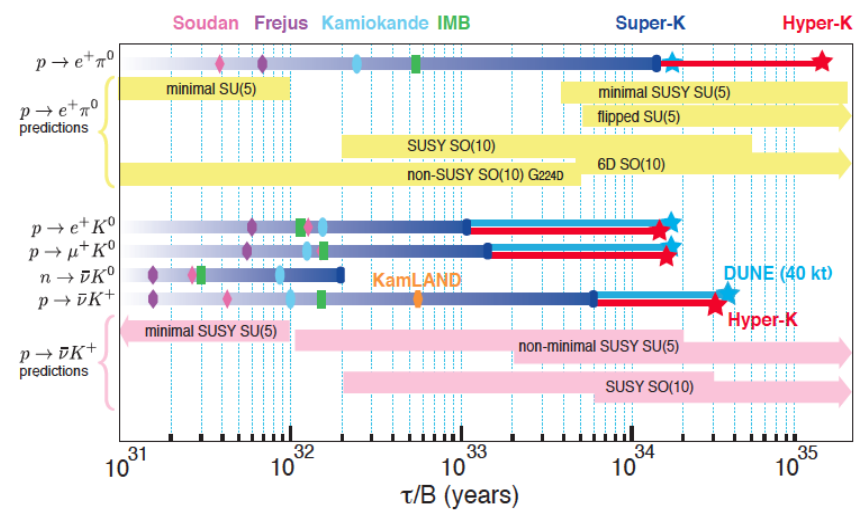
\includegraphics[width=\textwidth]{Chapter-2/Images/PDKExperimentalLImit.png}
\caption{Proton decay lifetime limits from passed and future experiments.}
\label{fig:PDKExperimentalLImit}
\end{figure}


%\subsection{Non-Accelerator Physics Program}
%\subsection{Rare Decay Searches: Experimental Limit}
%\subsection{Nucleon Decay Detection in LAr}
\subsection{Enabling the next generation of discoveries: LArIAT}\label{ch:LArIATIntro}
LArIAT, a small LArTPC in a test beam,  is designed to perform an extensive physics campaign centered on charged particle cross section measurements while characterizing the detector performance for future LArTPCs. Since LArTPCs represent the most advanced experiments for physics at the Intensity Frontier, their complex technology needs a thorough calibration and dedicated measurements of some key quantities to achieve the precision required for the next generation of discoveries.  LArIAT's goal is to provide such calibration and dedicated measurements. The LArIAT LArTPC is deployed in a dedicated calibration test beamline at Fermilab. We use the LArIAT beamline to characterize the charge particles before they enter the TPC: the particle type and initial momentum is known from beamline information. The precise calorimetric energy reconstruction of the LArTPC technology enables the measurement of the total differential cross section for  tagged hadrons. 
The Pion-Nucleus and Kaon-Nucleus total hadronic interaction cross section have never been measured before in argon and they are a fundamental step to shed light on light meson interaction in nuclei per se, while providing a key input to neutrino physics and proton decay studies in future LArTPC experiments like SBN and DUNE. 

In order to showcase LArIAT's utility to SBN and DUNE, we illustrate briefly two comparisons as examples: one regarding neutrino interactions and the second regarding proton decay studies.\\
The left side of figure \ref{fig:NuSimulation} shows the distribution of products in momentum spectrum and particle type as simulated in a $\nu_e$ CC interaction in DUNE (according to \cite{LeiguideOliveira:1953730}); the range of these distribution is to compare with  the momentum distribution of light particles in the LArIAT beamline -- shown on the right side of figure \ref{fig:NuSimulation}. The momentum spectrum in the LArIAT beamline for electrons, muons and pions -- the most abundant particles produced in  a $\nu_e$ CC interaction -- covers a wide range of the expected momentum distribution in a neutrino event.


The signature of a proton decay event in the ``LAr golden mode" is the presence of a single kaon of about 400 MeV in the detector; the momentum spectrum of the kaon pre and post FSI in such an event as simulated by GENIE is shown on the left side of figure \ref{fig:PDKGENIE}. The right side of figure \ref{fig:PDKGENIE} shows the momentum spectrum of kaons in the LArIAT beamline. Kaons arriving to the LArIAT TPC are ideal for proton decay studies, since their momentum in the beamline is just above the typical momentum for kaons in a proton decay event: the majority of LArIAT kaons slow down in the TPC enough to enter the desired momentum window.


\begin{figure}[hbpt]
\centering
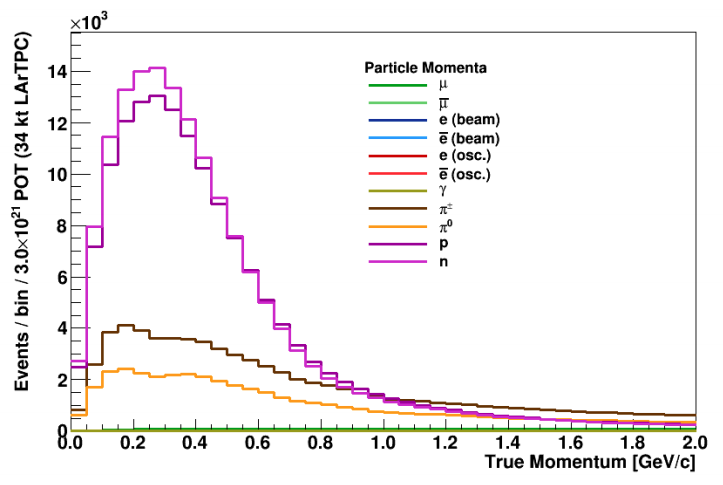
\includegraphics[width=0.45\textwidth]{Chapter-2/Images/NueCCSim.png}	
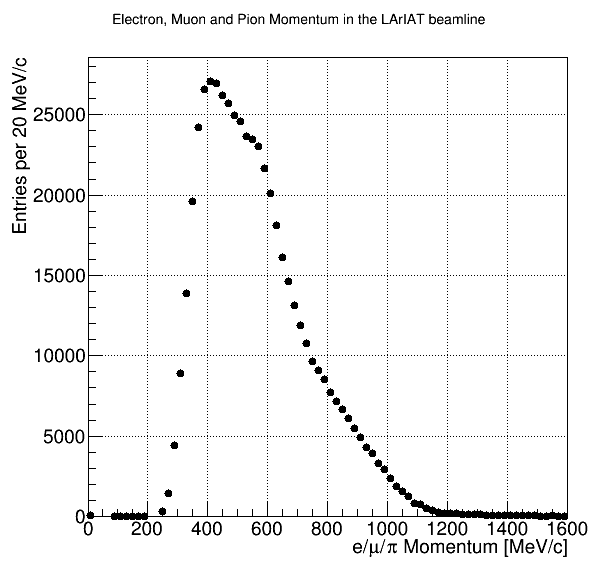
\includegraphics[width=0.45\textwidth]{Chapter-2/Images/momentumPiMuE.png}
\put(-88,155){\bf\tiny{LArIAT Preliminary}}
\caption{$Left$. Simulation of the products of a $\nu_e$ CC interaction in DUNE, both in particles type and momentum. \\
$Right$. Momentum spectrum for low mass particles ($e,\mu,\pi$) in the LArIAT beamline,  negative tune, Run II, Picky Tracks see section \ref{sec:MWPCfunc}. }
\label{fig:NuSimulation}
\end{figure}


\begin{figure}[hbpt]
\centering
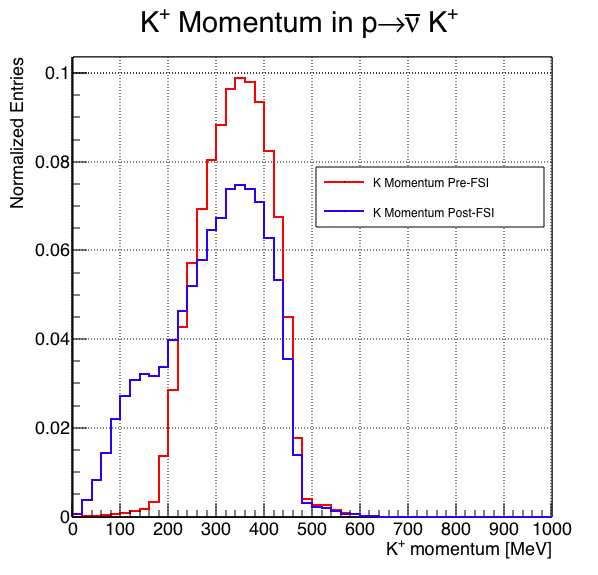
\includegraphics[width=0.45\textwidth]{Chapter-2/Images/pdkGenie.png}	
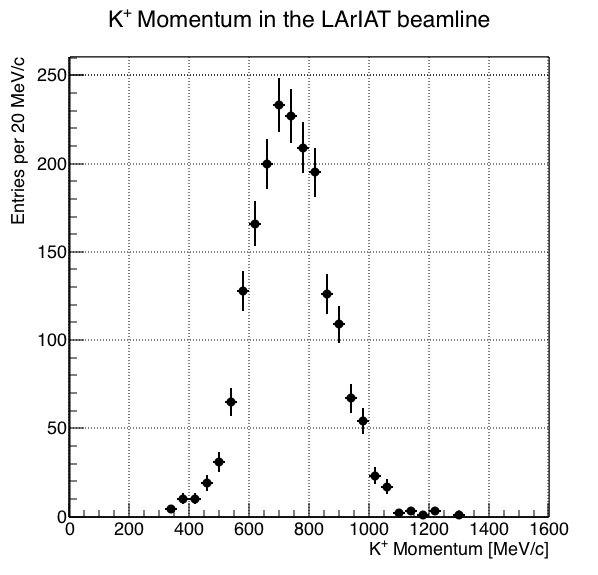
\includegraphics[width=0.45\textwidth]{Chapter-2/Images/MomentumKaonsDatabeamline.png}
\put(-290,155){\bf\tiny{LArIAT Preliminary}}
\put(-95,155){\bf\tiny{LArIAT Preliminary}}
\caption{$Left$. Momentum of the kaon outgoing a proton decay $p\rightarrow K^+\bar\nu$ event as simulated by the Genie 2.8.10 event generator in argon. The red line represents the kaon momentum distribution before undergoing the simulated final state interaction inside the argon nucleus, while the blue line represents the momentum distribution after FSI.\\
$Right$. Positive Kaon momentum spectrum in the LArIAT beamline,  positive tune, Run II, Picky Tracks see section \ref{sec:MWPCfunc}. }
\label{fig:PDKGENIE}
\end{figure}


